
\begin{figure*}[t]
  \centering
    {\footnotesize
       \begin{tabular}{p{3.4cm}p{3.4cm}p{3.6cm}p{3.6cm}}
        % \multicolumn{4}{c}{\textbf{VG: sandwich}}\\
\raisebox{-\totalheight}{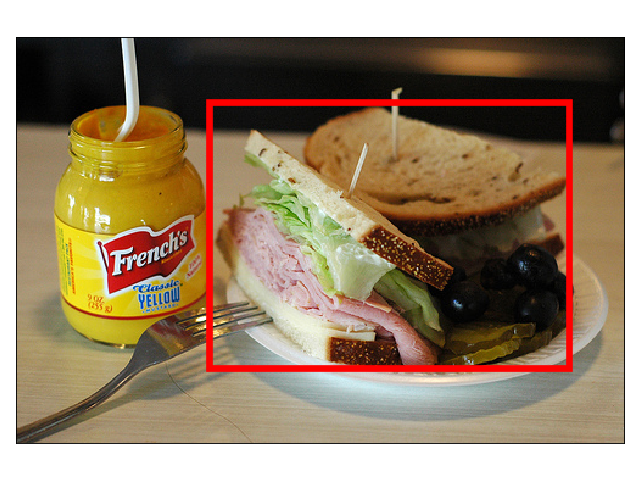
\includegraphics[width=0.9\linewidth]{figures/2339876_3928476_supercat_unique.png}} &
				\raisebox{-\totalheight}{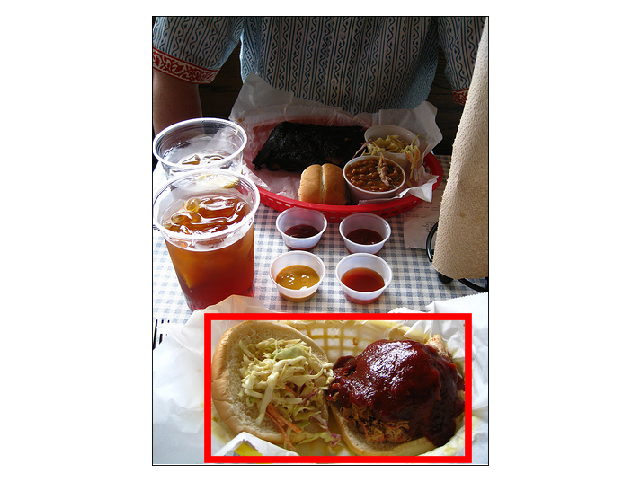
\includegraphics[width=0.9\linewidth]{figures/2379889_1353176_supercat_unique.png}} &
				\raisebox{-\totalheight}{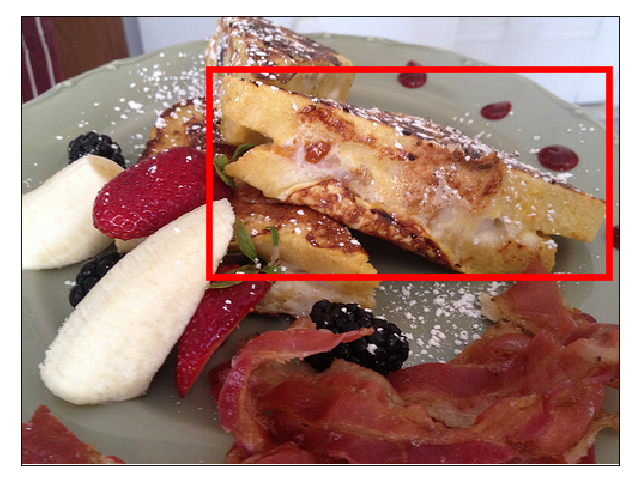
\includegraphics[width=0.9\linewidth]{figures/2394266_465678_singleton_obj.png}} &
				\raisebox{-\totalheight}{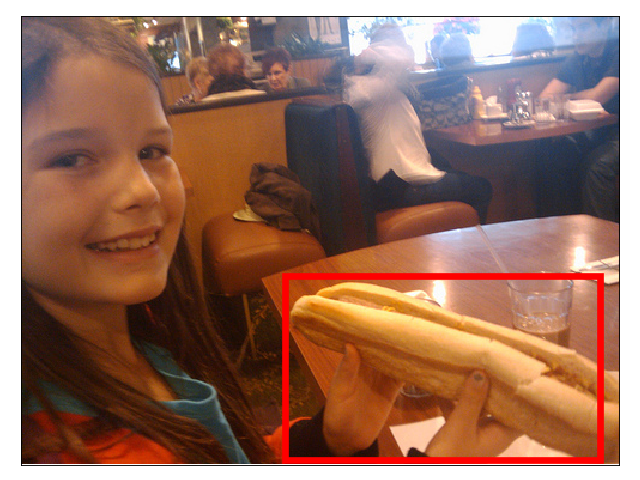
\includegraphics[width=0.9\linewidth]{figures/2386509_681763_supercat_unique.png}} \\

\textbf{A:} sandwich (34) &
\textbf{B:} sandwich (15), basket (6), food (5), burger (2),  hamburger (2),  meal (2) &
 \textbf{C:} food (10), sandwich (8), toast (5), french toast (4), dessert (2), breakfast (2) &
 \textbf{D:} hotdog (14), food (7), bun (4), sandwich (3),  bread (2)\\

        % \multicolumn{4}{c}{\textbf{VG: bridge} } \\
\raisebox{-\totalheight}{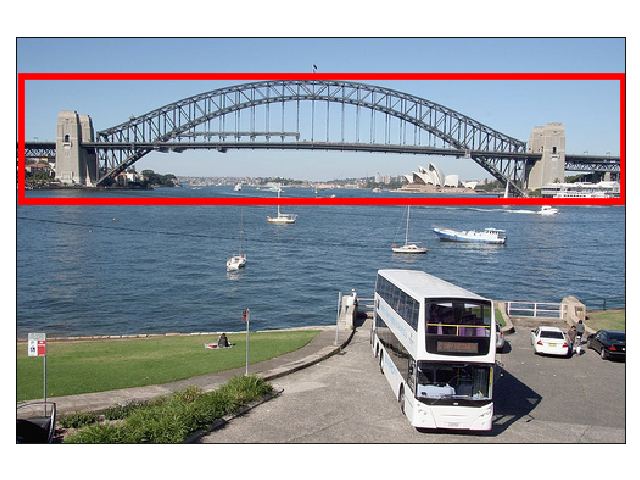
\includegraphics[width=0.9\linewidth]{figures/2341667_2006329_singleton_obj.png}} &
				\raisebox{-\totalheight}{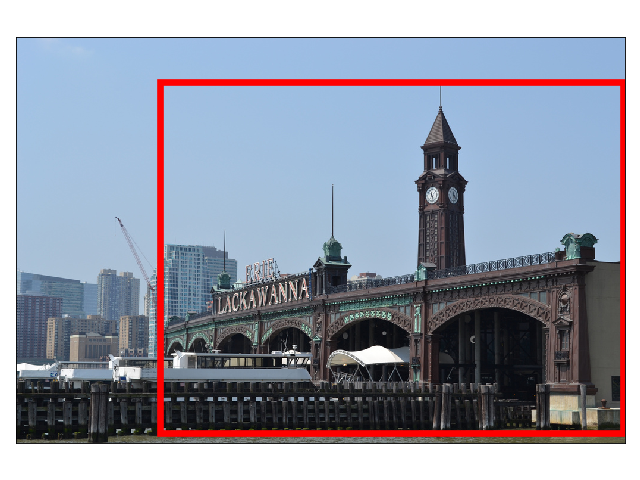
\includegraphics[width=0.9\linewidth]{figures/1592509_1610006_singleton_obj.png}} &
				\raisebox{-\totalheight}{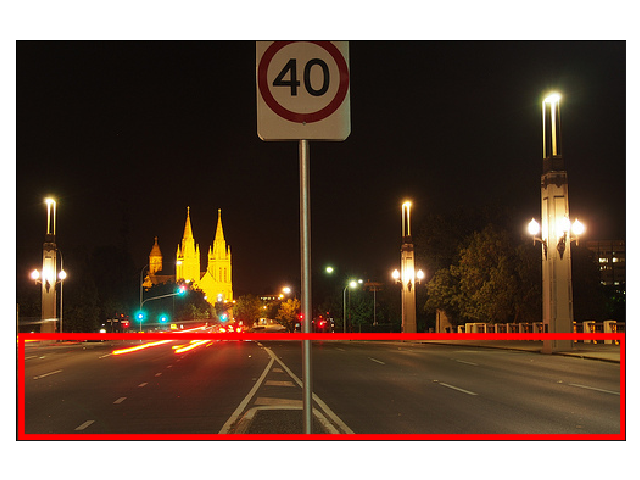
\includegraphics[width=0.9\linewidth]{figures/2384683_1306430_singleton_obj.png}} &
				\raisebox{-\totalheight}{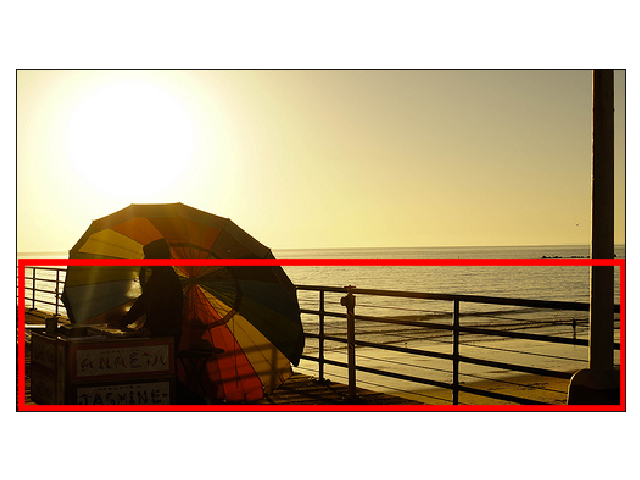
\includegraphics[width=0.9\linewidth]{figures/2412972_3494120_singleton_obj.png}} \\

 \textbf{E:} bridge (35)  &
 \textbf{F:} bridge (20),  building (11)  &
 \textbf{G:} street (16), road (15), bridge (3) &
 \textbf{H:} pier (6), railing (5), dock (5), bridge (5), fence (4), rail (3), boardwalk (3)\\

        % \multicolumn{4}{c}{\textbf{VG: bed}}\\
\raisebox{-\totalheight}{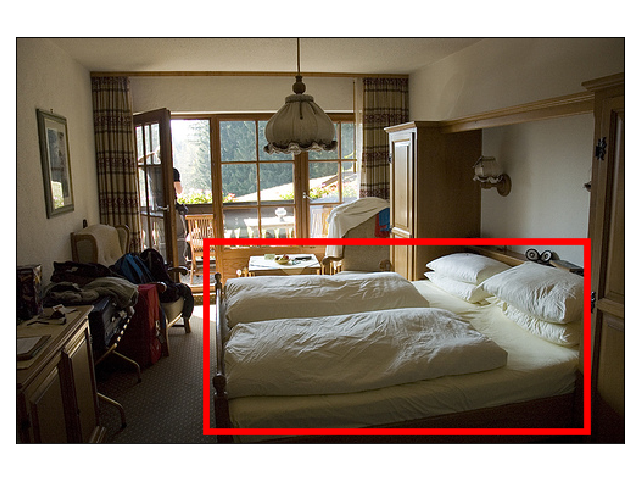
\includegraphics[width=0.9\linewidth]{figures/2321254_3438076_singleton_obj.png}} &
				\raisebox{-\totalheight}{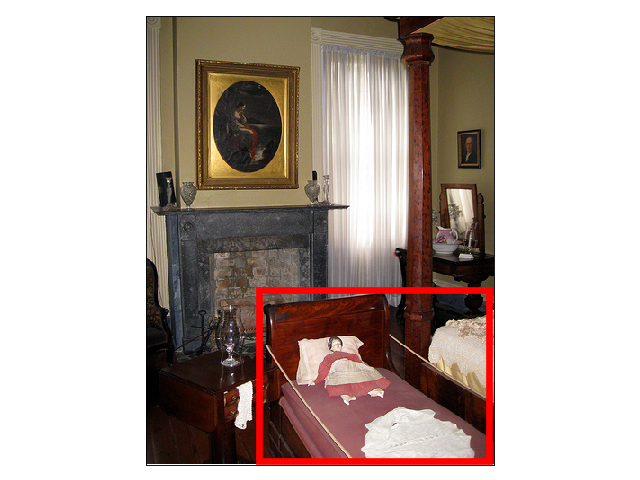
\includegraphics[width=0.9\linewidth]{figures/2324306_3412337_singleton_obj.png}} & 
				\raisebox{-\totalheight}{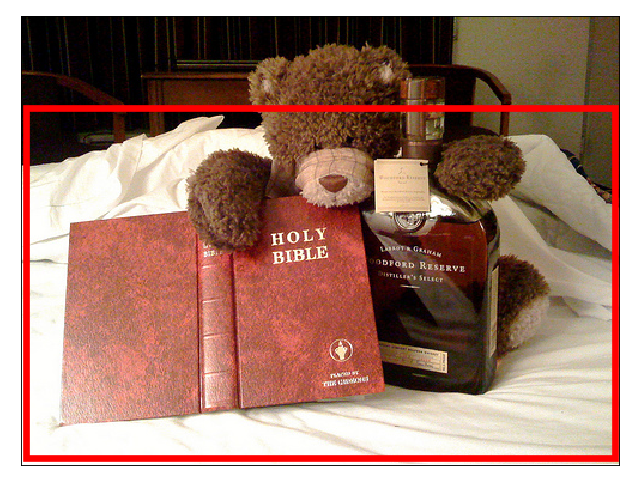
\includegraphics[width=0.9\linewidth]{figures/2342811_3485104_singleton_obj.png}} &
				\raisebox{-\totalheight}{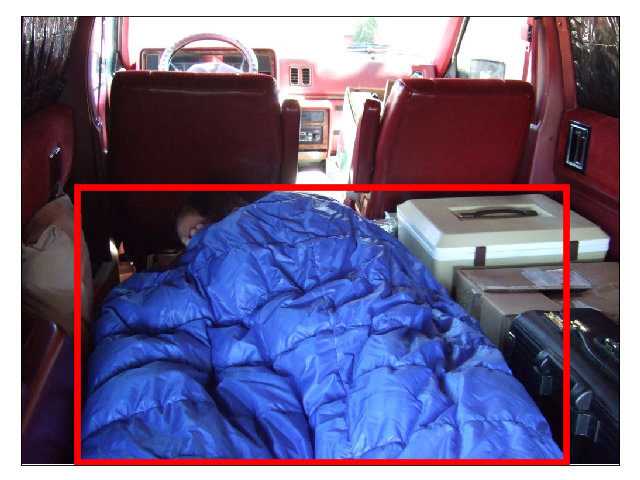
\includegraphics[width=0.9\linewidth]{figures/498222_3135415_singleton_obj.png}} \\

 \textbf{I:} bed (36)  &
 \textbf{J:} bed (16), bench (6), crib (5) &
 \textbf{K:} bed (17), book (6), table (4), toy (3), bible (2), doll (2) &
 \textbf{L:} bed (12), sleeping bag (9), blanket (7), bed sheet (5)\\

       \end{tabular}
    }
  \caption{Examples for \vgenome images labeled \word{sandwich}, \word{bridge}, and \word{bed} (first, second, last row, respectively) with higher to lower agreement in ManyNames.} 
    %Names that have a hierarchical relation to the \vgenome synset in WordNet are underlined.}
	\label{fig:ex-high-low-agreement}
\end{figure*}



% \begin{figure*}[t]
%   \centering
%     {\footnotesize
%       \begin{tabular}{p{2.2cm}p{2.6cm}p{2.6cm}p{2.6cm}}
%         % \multicolumn{4}{c}{\textbf{VG: sandwich}}\\
% \raisebox{-\totalheight}{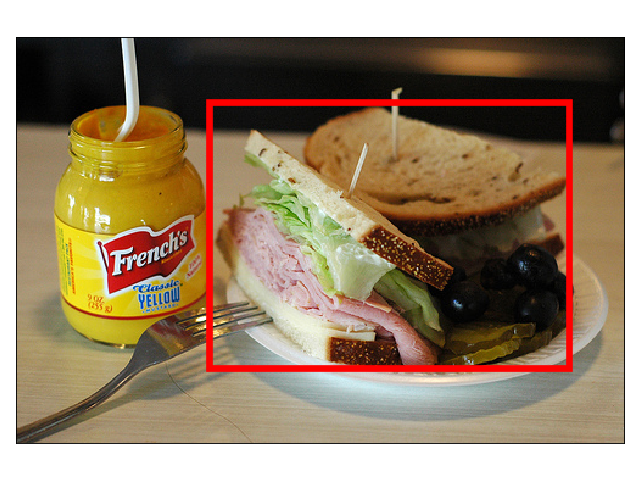
\includegraphics[width=0.9\linewidth]{figures/2339876_3928476_supercat_unique.png}} \textbf{A:} sandwich (34) &
% 				\raisebox{-\totalheight}{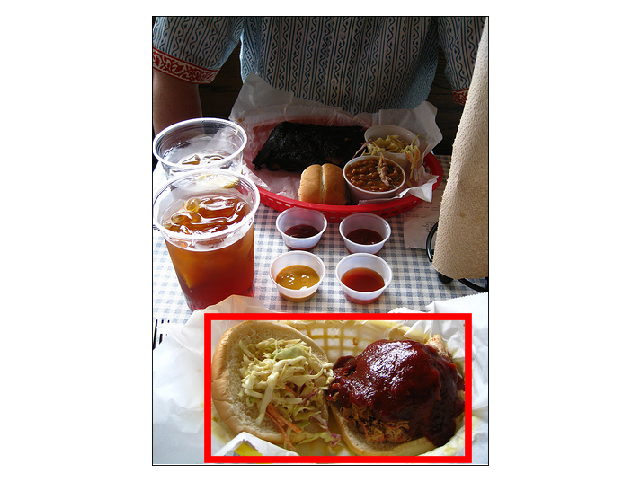
\includegraphics[width=0.9\linewidth]{figures/2379889_1353176_supercat_unique.png}} \textbf{B:} sandwich (15), basket (6), food (5), burger (2),  hamburger (2),  meal (2) &
% 				\raisebox{-\totalheight}{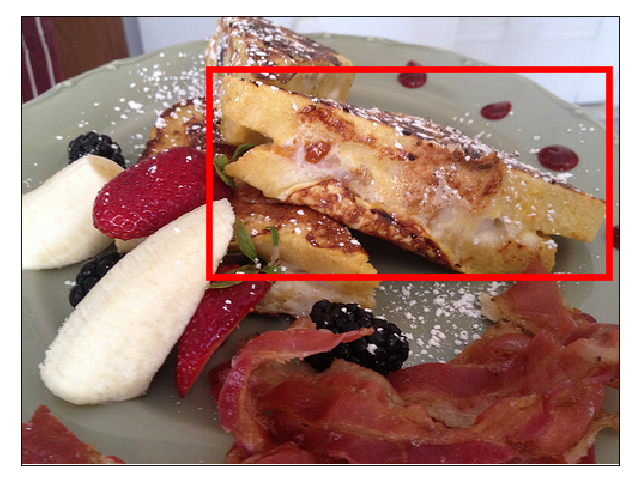
\includegraphics[width=0.9\linewidth]{figures/2394266_465678_singleton_obj.png}} \textbf{C:} food (10), sandwich (8), toast (5), french toast (4), dessert (2), breakfast (2) &
% 				\raisebox{-\totalheight}{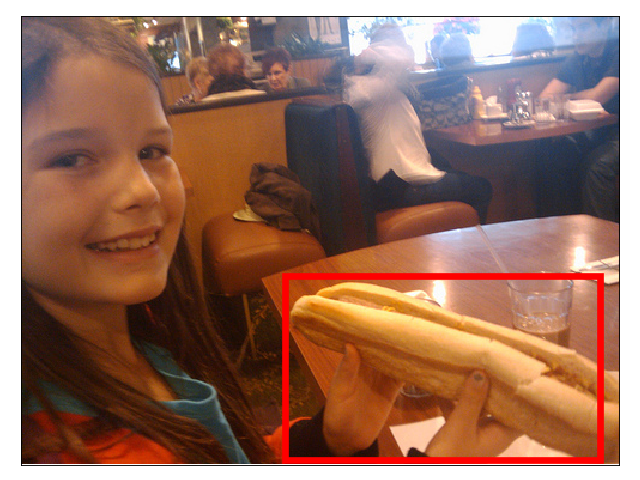
\includegraphics[width=0.9\linewidth]{figures/2386509_681763_supercat_unique.png}} \textbf{D:} hotdog (14), food (7), bun (4), sandwich (3),  bread (2) \\

%         % \multicolumn{4}{c}{\textbf{VG: bridge} } \\
% \raisebox{-\totalheight}{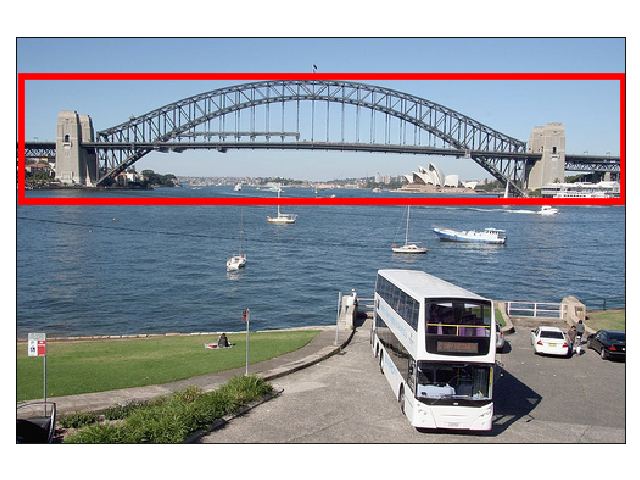
\includegraphics[width=0.9\linewidth]{figures/2341667_2006329_singleton_obj.png}} \textbf{E:} bridge (35)  &
% 				\raisebox{-\totalheight}{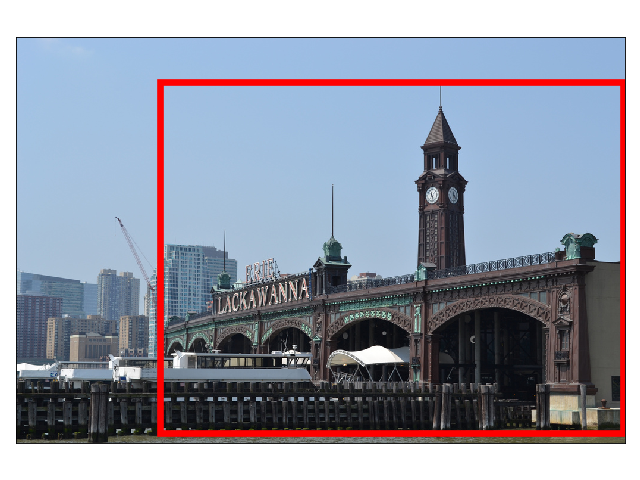
\includegraphics[width=0.9\linewidth]{figures/1592509_1610006_singleton_obj.png}} \textbf{F:} bridge (20),  building (11)  &
% 				\raisebox{-\totalheight}{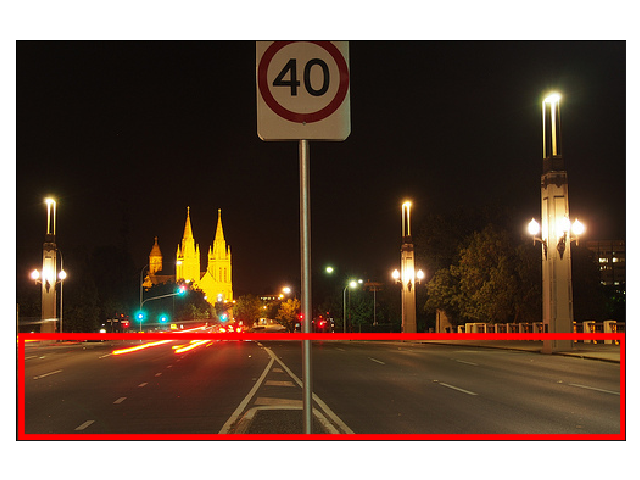
\includegraphics[width=0.9\linewidth]{figures/2384683_1306430_singleton_obj.png}} \textbf{G:} street (16), road (15), bridge (3) &
% 				\raisebox{-\totalheight}{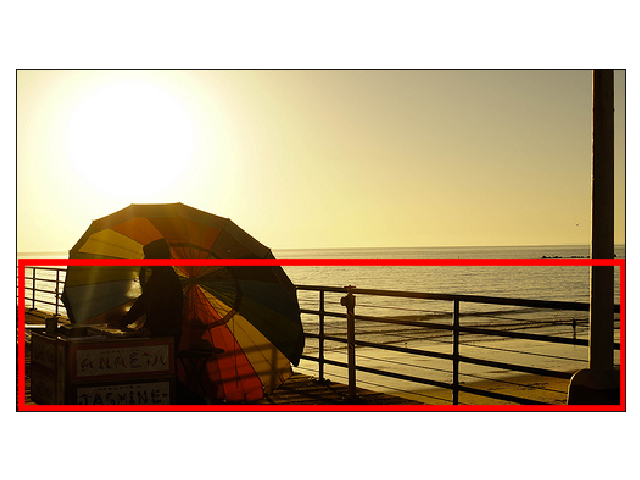
\includegraphics[width=0.9\linewidth]{figures/2412972_3494120_singleton_obj.png}} \textbf{H:} pier (6), railing (5), dock (5), bridge (5), fence (4), rail (3), boardwalk (3)\\
%         % \multicolumn{4}{c}{\textbf{VG: bed}}\\
% \raisebox{-\totalheight}{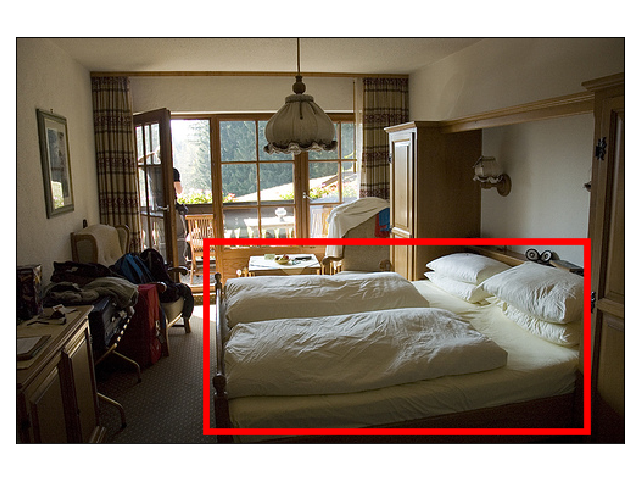
\includegraphics[width=0.9\linewidth]{figures/2321254_3438076_singleton_obj.png}} \textbf{I:} bed (36)  &
% 				\raisebox{-\totalheight}{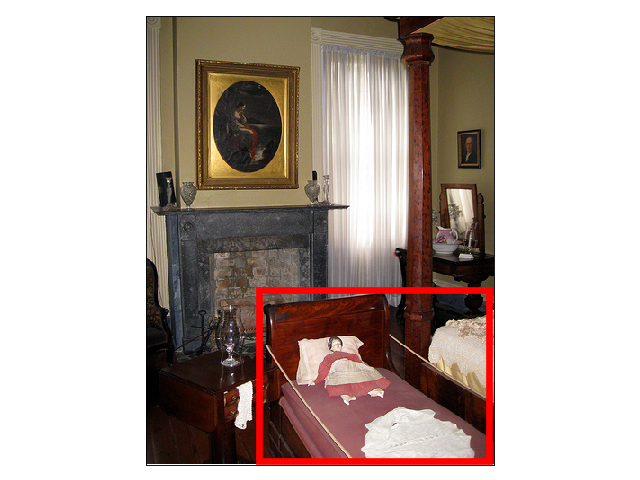
\includegraphics[width=0.9\linewidth]{figures/2324306_3412337_singleton_obj.png}} \textbf{J:} bed (16), bench (6), crib (5) &
% 				\raisebox{-\totalheight}{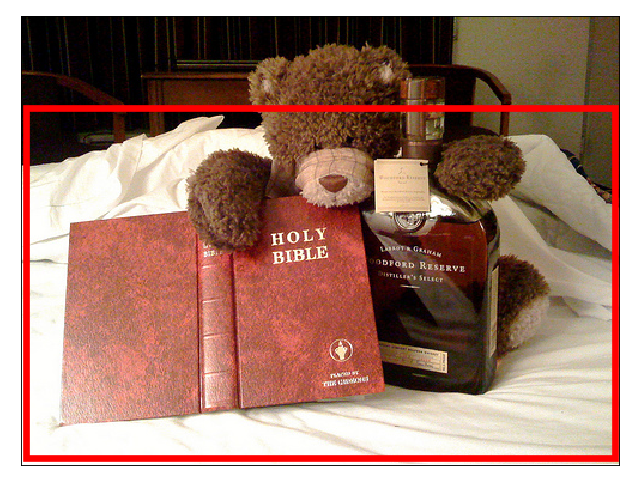
\includegraphics[width=0.9\linewidth]{figures/2342811_3485104_singleton_obj.png}} \textbf{K:} bed (17), book (6), table (4), toy (3), bible (2), doll (2) & 
% 				\raisebox{-\totalheight}{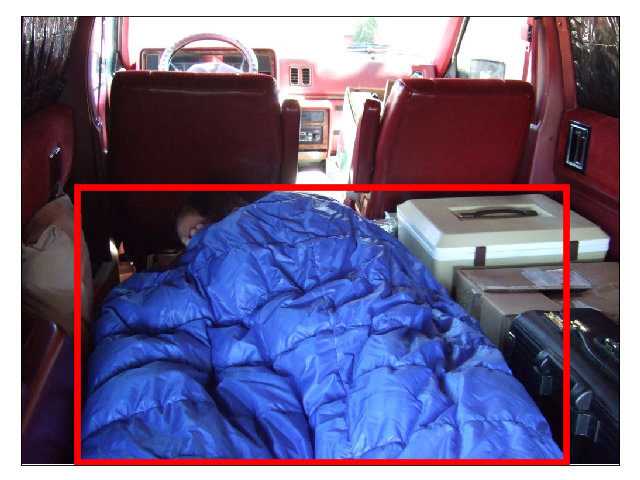
\includegraphics[width=0.9\linewidth]{figures/498222_3135415_singleton_obj.png}} \textbf{L:} bed (12), sleeping bag (9), blanket (7), bed sheet (5)\\
%       \end{tabular}
%     }
%   \caption{Examples for \vgenome images labeled \word{sandwich}, \word{bridge}, and \word{bed} (first, second, last row, respectively) with higher to lower agreement in ManyNames.} 
%     %Names that have a hierarchical relation to the \vgenome synset in WordNet are underlined.}
% 	\label{fig:ex-high-low-agreement}
% \end{figure*}



%%% Local Variables:
%%% mode: latex
%%% TeX-master: "lrec2020naming"
%%% End:
